\documentclass[12pt,a4paper,leqno]{article}
\usepackage[utf8]{inputenc}
\usepackage[T1]{fontenc}
\usepackage[english]{babel}
\usepackage{amsmath}
\usepackage{amsfonts}
\usepackage{amssymb}
\usepackage{graphicx}
\usepackage{minted}
\usepackage{hyperref}
\hypersetup{
	colorlinks=true,
	linkcolor=blue
}

\graphicspath{{./images}}

\title{Predict Parkinson Disease using wearable data}
\author{Aloi Alfredo, Riccio Francesco}

\begin{document}
	
	\maketitle
	
	\begin{abstract}
		This is a project for the Deep Learning course held in the Master Degree in Computer Science of Università degli Studi della Calabria.
	\end{abstract}
	
	\newpage
	
	\tableofcontents
	
	\newpage
	
	\section{Introduction}
	Parkinson disease, the second most neurological disorder that causes significant disability, reduces the quality of life and has no cure. Approximately, 90\% affected people with Parkinson have speech disorders. Deep learning has the potential to give valuable information after processing that can be discovered through deep analysis and efficient processing of data by decision makers. The main problem is the identification of OFF symptoms perceived by the study subject with reasonable accuracy from real-world data collected. OFF periods are times when Parkinson’s disease medication, namely levodopa, is not working optimally. As a result, symptoms return. OFF periods can include both motor symptoms, such as tremor and rigidity, and non-motor symptoms, such as anxiety. The goal is to consolidate data collection by identifying the most important variables to solve the problem.
	
	\newpage
	
	\section{Task 1: next value prediction}
	We have 3 time series (X, Y, Z) recorded each 10 seconds. For the first sub-task we consider, for each time series, sequences of five minutes (\mintinline[breaklines]{python}|window_size = 30|) every one minute (\mintinline[breaklines]{python}|window_shift = 6|), predicting the next value in the series. The evaluation metric is the Mean Absolute Error, in particular we have to go below:
	\begin{itemize}
		\item 81.06 for X;
		\item 85.26 for Y;
		\item 79.94 for Z.
	\end{itemize}
	We then choose, for the second sub-task, the one time series with the worst value of the evaluation metric, looking for a better combination of window size/window shift.
	
	\subsection{Data understanding and preparation}
	We have two files, \mintinline[breaklines]{python}|train.csv| and \mintinline[breaklines]{python}|test.csv|, each one containing three columns, representing the three time series X, Y and Z. The \mintinline[breaklines]{python}|test.csv| file will be used for the evaluation, while the \mintinline[breaklines]{python}|train.csv| file, that contains 144910 rows, will be used for the training part.
	
	Since the three time series to be used in the training steps are inside one single dataset, we start the preparation of our data by first splitting it into the three different time series. For each one of the generated time series:
	\begin{enumerate}
		\item we produce a set of sequences, basing ourselves on the aforementioned window size and window shift, with the corresponding labels, representing the element that follows each sequence in the series;
		\item we normalize the values inside the produced sequences using a Standard scaler, which scales the data according to a Normal distribution;
		\item we, additionally, split the produced sequences to obtain training and validation sets to use in the training step, using a ratio of 80:20.
	\end{enumerate}
	
	\subsection{Modeling}
	We choose to build a neural architecture starting with three LSTM layers followed by four Dense layers, with the last one made of just one neuron, which is our output. Between each layer of the architecture we choose to put a dropout layer to mitigate the overfitting bias. We employ a Hyperband tuner to make the choice of the best model parameters for us.
	\begin{figure}
		\centering
		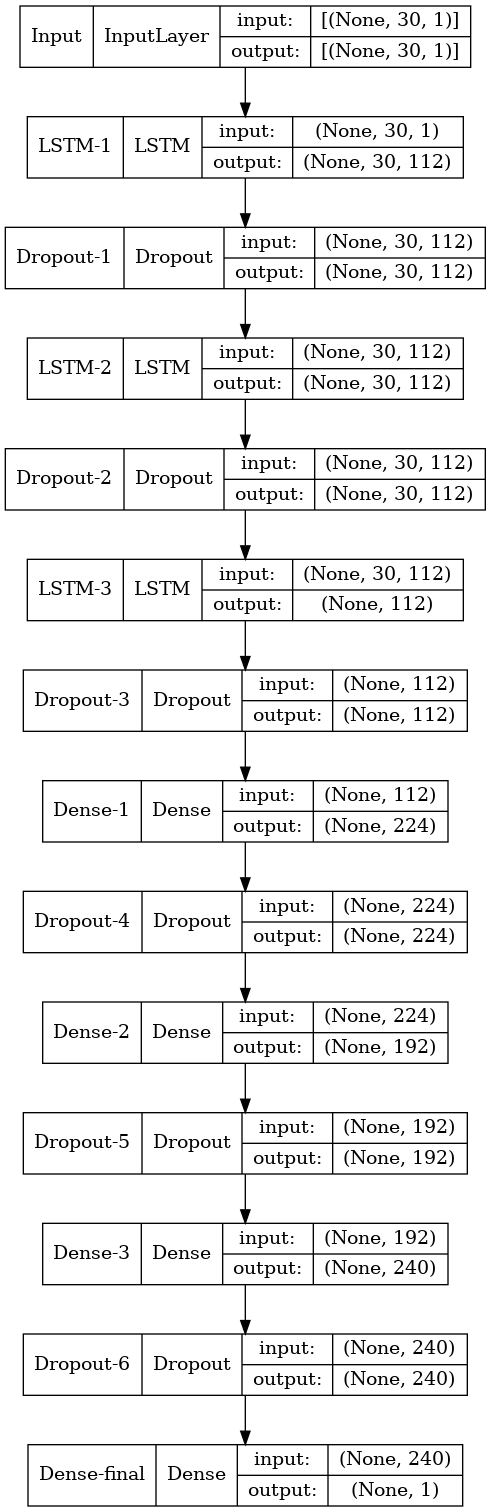
\includegraphics[height=0.9\textheight]{/task_1.1/x_model.png}
		\caption{The model for Z time series}
		\label{task_1.1/x_model}
	\end{figure}
	\begin{figure}
		\centering
		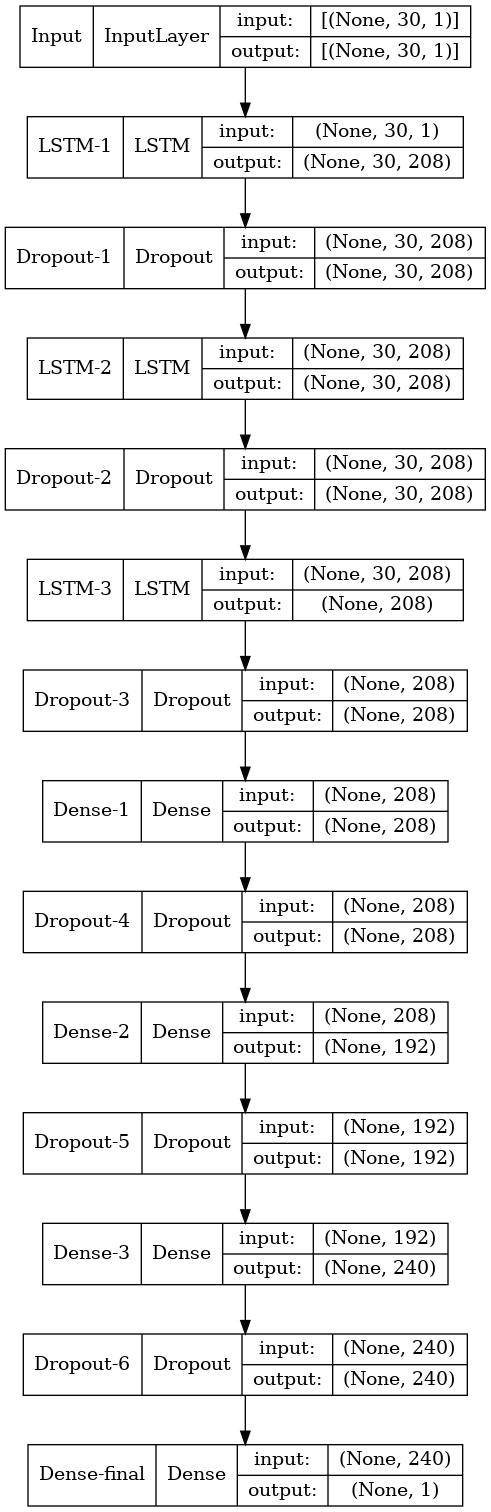
\includegraphics[height=0.9\textheight]{/task_1.1/y_model.png}
		\caption{The model for Z time series}
		\label{task_1.1/y_model}
	\end{figure}
	\begin{figure}
		\centering
		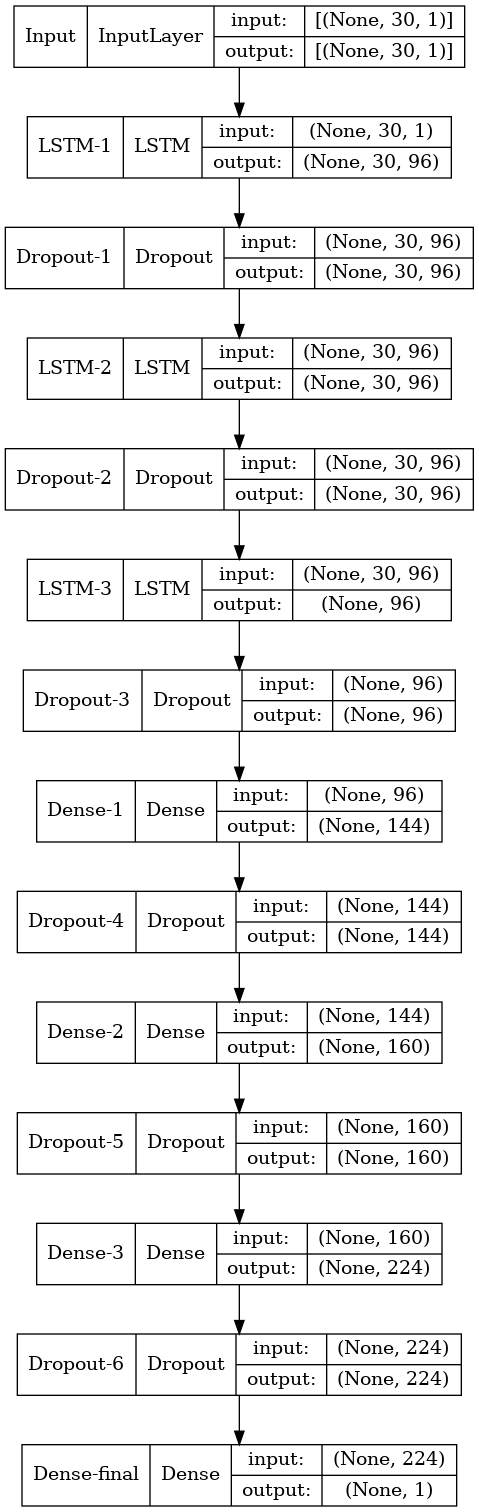
\includegraphics[height=0.9\textheight]{/task_1.1/z_model.png}
		\caption{The model for Z time series}
		\label{task_1.1/z_model}
	\end{figure}
	Next, we fit our models for 25 epochs using a batch size of 32, keeping track of the evaluation metric score of the validation data used during training, in order to save only the best behaving model; this is done using a Model Checkpoint as callback to the fitting process.
	\begin{figure}[h]
		\centering
		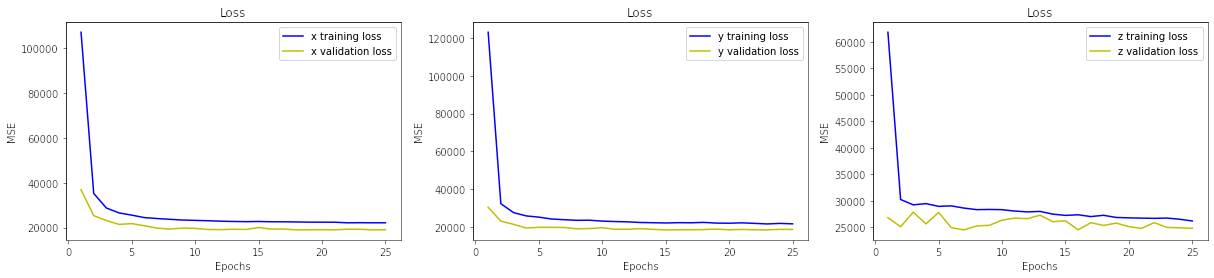
\includegraphics[width=\linewidth]{/task_1.1/losses.png}
		\caption{The losses during training}
		\label{task_1.1/losses}
	\end{figure}
	\begin{figure}[h]
		\centering
		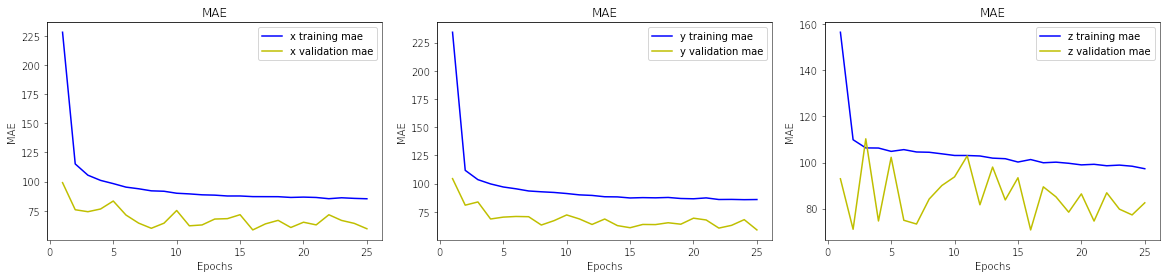
\includegraphics[width=\linewidth]{/task_1.1/maes.png}
		\caption{The MAE during training}
		\label{task_1.1/maes}
	\end{figure}
	
	\subsection{Evaluation}
	Looking at the plots regarding the loss (\autoref{task_1.1/losses}), we can observe how in the first epochs the models learn very quickly, suffering a sudden slowdown in the following epochs, but, anyway, the learning curve appears to be quite smooth for each time series. On the other hand, we can notice, in the plots regarding the Mean Absolute Error (\autoref{task_1.1/maes}), that each time series has an irregular behaviour, especially the Z time series, with a high variability in the values of said metric during training.
	
	To evaluate our models, we first have to apply the same preprocessing steps also to the test dataset, namely: splitting of the different time series, generation of sequences and normalization.
	\begin{table}
		\centering
		\begin{tabular}{|c|c|c|}
			\hline
			& \textbf{Target} & \textbf{Actual} \\ 
			\hline
			\hline
			X & 81.06 & \textbf{77.62} \\
			Y & 85.26 & \textbf{84.31} \\
			Z & 79.94 & \textbf{78.39} \\
			\hline
		\end{tabular}
		\caption{Testing results obtained}
		\label{task_1.1/evaluation}
	\end{table}
	Concerning the results obtained after testing (\autoref{task_1.1/evaluation}), these are quite good, all the evaluation metrics respect the set objective values. In particular, with regards to the X time series, we are far below the target threshold (77.62 compared to 81.06), while for the other two the difference is smaller (84.31 and 78.39 compared to, respectively, 85.26 and 79.94).	
	
	\subsection{Finding better parameters}
	The objective of this subtask is to try to improve the results obtained previously, for the Y time series. Specifically, we want to find a better combination of window size and window shift. To make this possible, we have defined a search space, consisting of five values for the window size (18, 24, 30, 36 and 42) and four values for the window shift (1, 3, 6, 9). For each combination of window size/window shift we fit the model and test it, saving the respective evaluation.
	\begin{figure}[h]
		\centering
		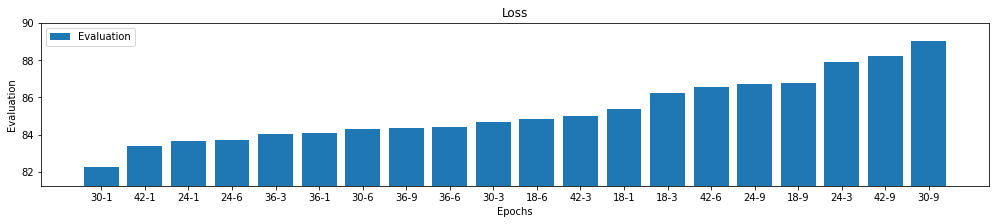
\includegraphics[width=\linewidth]{/task_1.2/evaluations.png}
		\caption{The evaluations for each combination}
		\label{task_1.2/evaluations_plot}
	\end{figure}
	\begin{table}
		\centering
		\begin{tabular}{|c|c|c|}
			\hline
			\textbf{Window size} & \textbf{Window shift} & \textbf{Score} \\ 
			\hline
			\hline
			18 & 1 & \textbf{85.35} \\
			18 & 3 & \textbf{86.21} \\
			18 & 6 & \textbf{84.83} \\
			18 & 9 & \textbf{88.20} \\
			24 & 1 & \textbf{83.65} \\
			24 & 3 & \textbf{87.91} \\
			24 & 6 & \textbf{83.71} \\
			24 & 9 & \textbf{86.74} \\
			30 & 1 & \textbf{82.24} \\
			30 & 3 & \textbf{84.69} \\
			30 & 6 & \textbf{84.31} \\
			30 & 9 & \textbf{89.01} \\
			36 & 1 & \textbf{84.06} \\
			36 & 3 & \textbf{84.03} \\
			36 & 6 & \textbf{84.41} \\
			36 & 9 & \textbf{84.37} \\
			42 & 1 & \textbf{83.36} \\
			42 & 3 & \textbf{85.01} \\
			42 & 6 & \textbf{86.55} \\
			42 & 9 & \textbf{88.20} \\
			\hline
		\end{tabular}
		\caption{Testing results obtained}
		\label{task_1.2/evaluations_table}
	\end{table}
	It can be noticed (\autoref{task_1.2/evaluations_plot}, \autoref{task_1.2/evaluations_table}) how models with a lower window shift tend to perform better, as opposed to those with a higher window shift, that do not perform in the same way.
	
	\subsection{All in one model}
	As an extra step we decide to build a model that takes as input the three time series at once, in order to see if we can obtain more accurate results. We use the same preprocessing approach used in the previous steps. Also here we use a Hyperband tuner to find the best parameters to use for our model, that is then fitted and tested.
	\begin{figure}
		\centering
		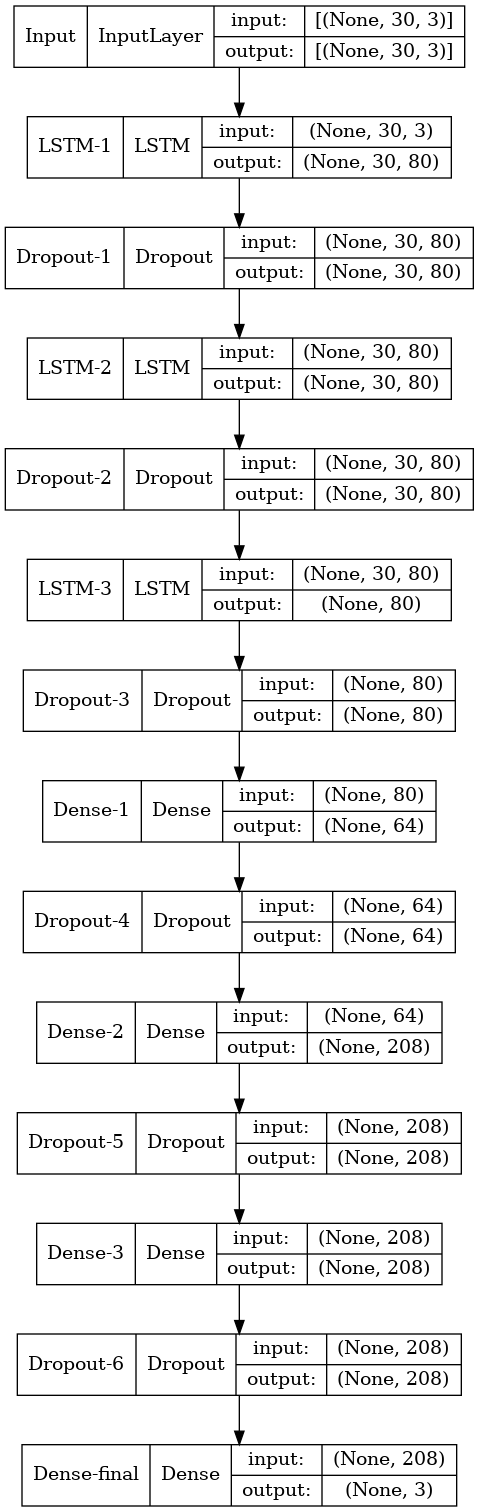
\includegraphics[height=0.9\textheight]{/task_1.3/model.png}
		\caption{The all in one model}
		\label{task_1.3/model}
	\end{figure}
	\begin{figure}
		\centering
		\includegraphics[width=\linewidth]{/task_1.3/loss&mae.png}
		\caption{The all in one model loss and MAE}
		\label{task_1.3/loss&mae}
	\end{figure}
	
	We are not surprised to see (\autoref{task_1.3/loss&mae}) that the plots are similar to the ones observed before. We can also notice that the model is now more easily keeping a not so high variation in evaluation metric during training, whereas before the values could vary wildly. In spite of this, the evaluation of the trained model on the test set has given a result of 93.86, that is higher than the worst result obtained by the same architecture using the three time series separately.
	
	\newpage
	
	\section{Task 2: anomaly detection}
	Given data from wearable devices, the goal is to identify anomalous events, like tremors, in a set of observations, that we refer to as OFF periods. Data are collected by patients with and without Parkinson’s Disease. Given the nature of the task, we opted for training a model capable of capturing the trend of the observations of people without Parkinson’s, in order to spot deviations from said trend, and thus the presence of OFF periods in the patient with Parkinson’s.
	
	\subsection{Data understanding and preparation}
	We have two files, \mintinline[breaklines]{python}|train.csv| and \mintinline[breaklines]{python}|test.csv|, each one containing seven columns. Features include:
	\begin{itemize}
		\item Identification of patient (\mintinline[breaklines]{python}|patient|);
		\item Accelerometer readings in the three axes (\mintinline[breaklines]{python}|x|, \mintinline[breaklines]{python}|y| and \mintinline[breaklines]{python}|z|);
		\item Heart rate (\mintinline[breaklines]{python}|heartRate|);
		\item Date and timestamp (\mintinline[breaklines]{python}|tsDate| and \mintinline[breaklines]{python}|timestamp|).
	\end{itemize}
	The \mintinline[breaklines]{python}|test.csv| file will be used for the detection of anomalies, while the \mintinline[breaklines]{python}|train.csv| file will be used for the training part. The training set is composed of control patients, i.e. volunteers without Parkinson’s Disease, there is a record each 1 second and there are missing values on the heart rate attribute (labeled with \mintinline[breaklines]{python}|-1|). The test set is composed by patients with Parkinson’s Disease and there is a record each 10 seconds. We decided to remove the missing values from the training set.
	\begin{figure}
		\centering
		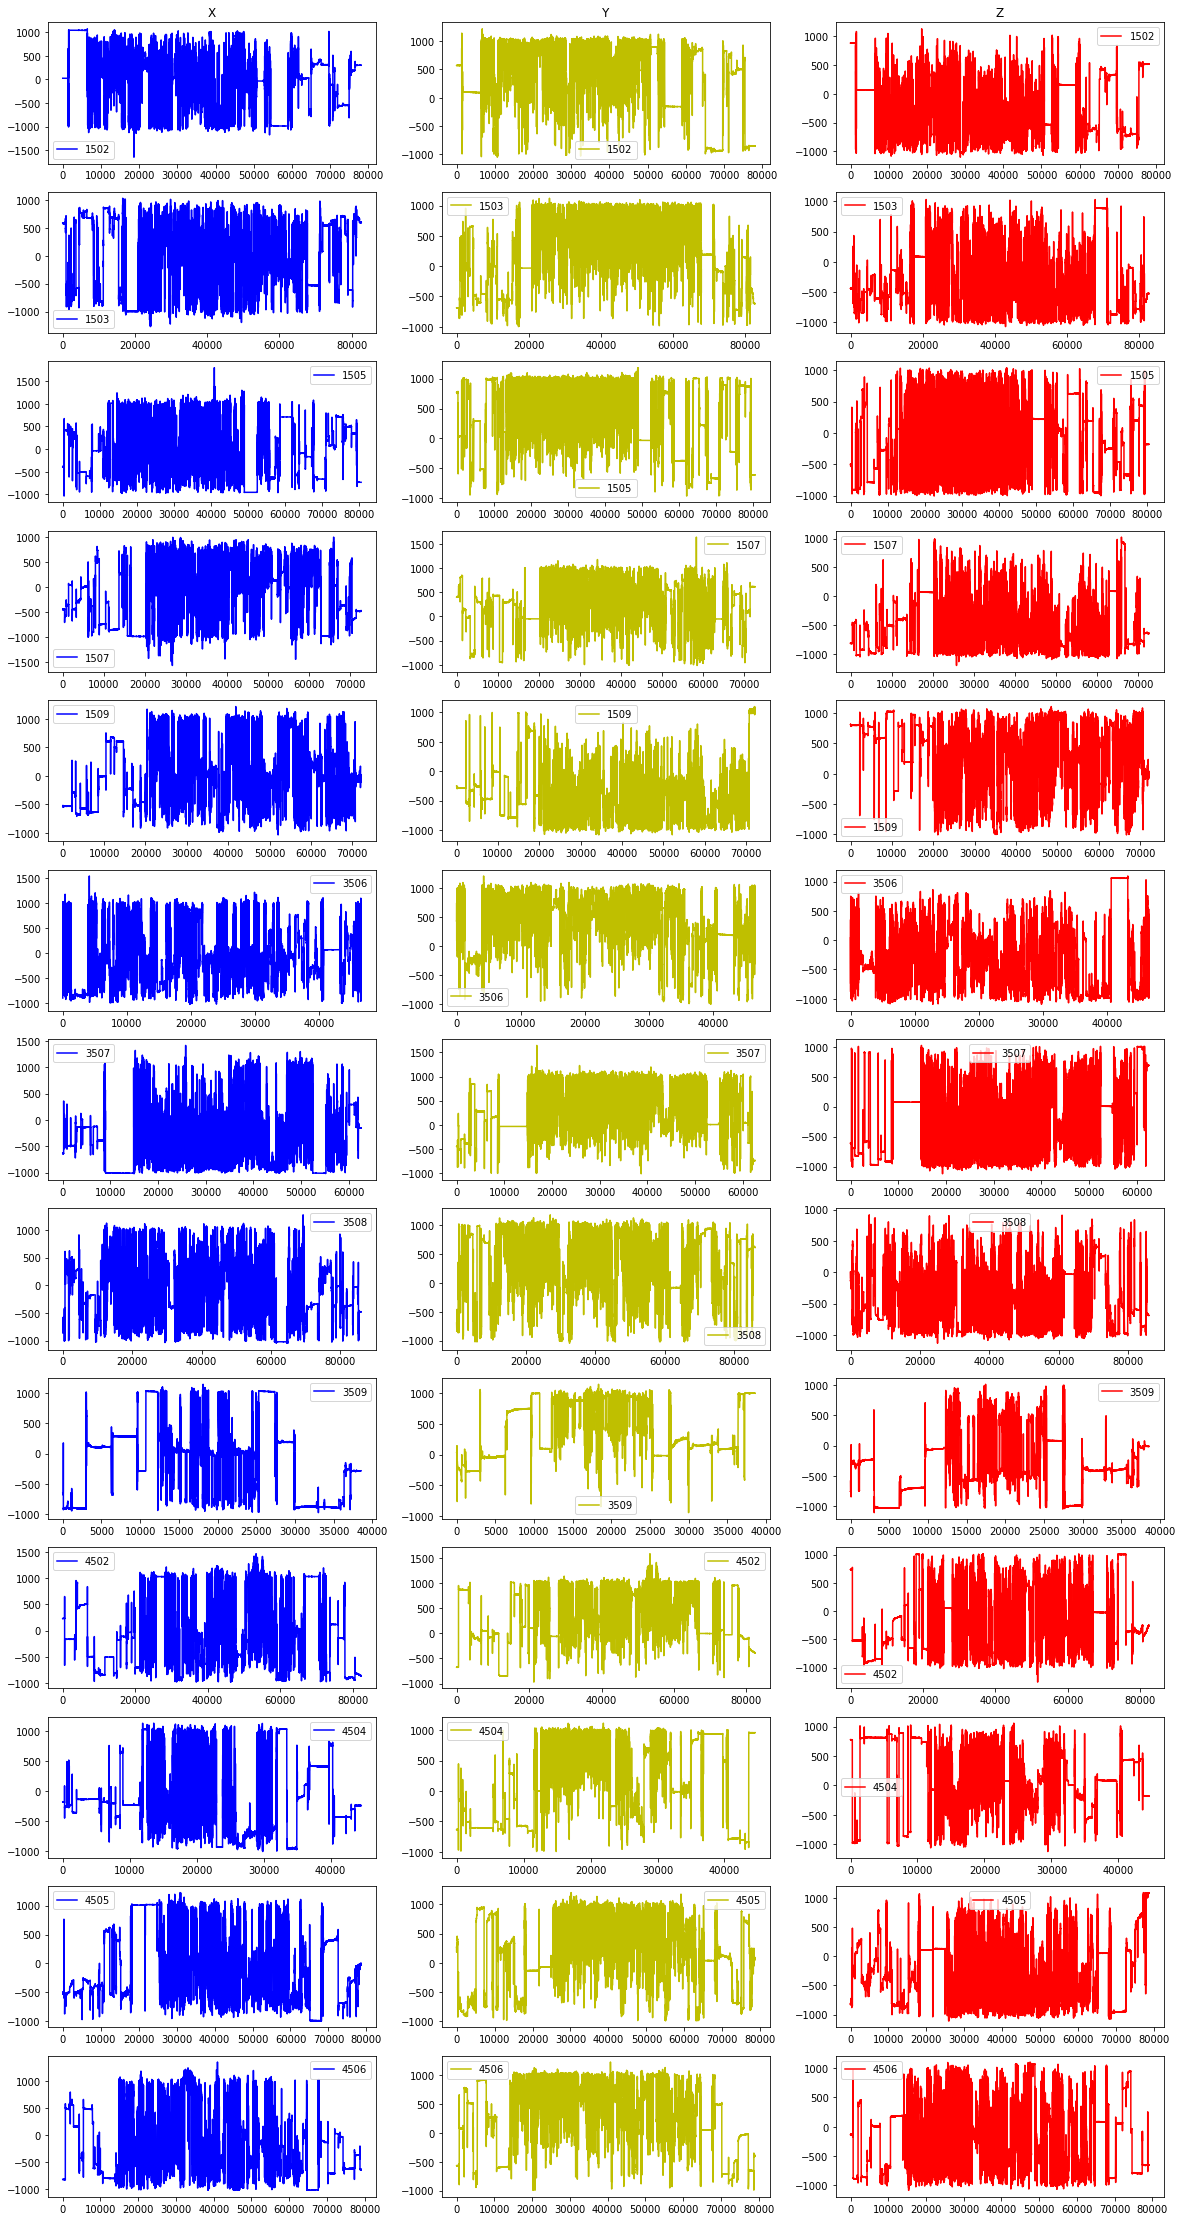
\includegraphics[height=0.9\textheight]{/task_2/spatial_coordinates.png}
		\caption{The X, Y and Z spatial coordinates for each patient}
		\label{task_2/spatial_coordinates}
	\end{figure}
	\begin{figure}
		\centering
		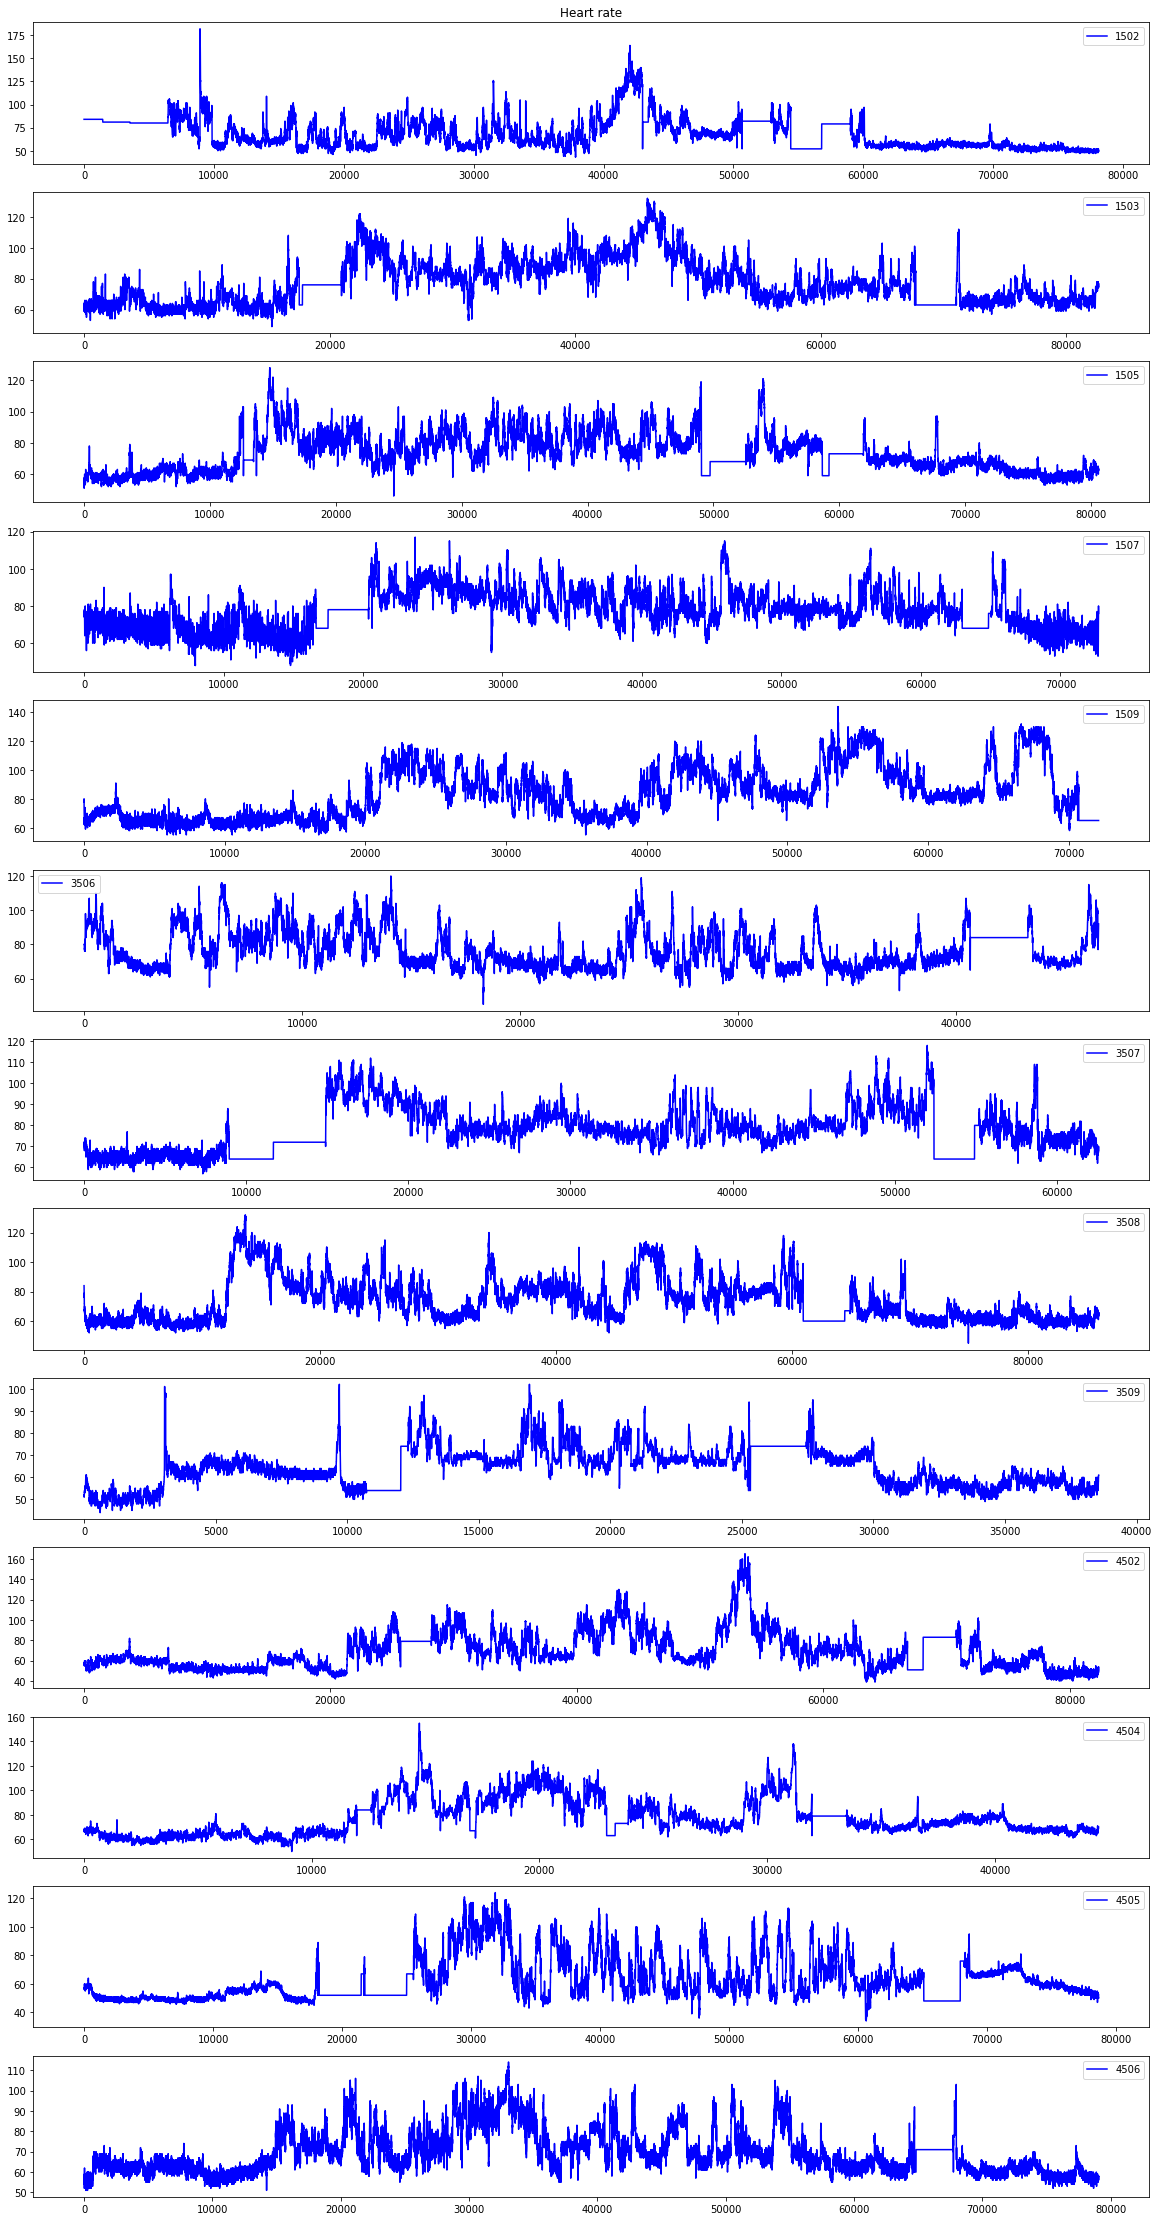
\includegraphics[height=0.9\textheight]{/task_2/heart_rate.png}
		\caption{The heart rate for each patient}
		\label{task_2/heart_rate}
	\end{figure}
	Given the granularity mismatch between training set and test set, we decided to resample the portion of training set regarding each patient, in order for them to appear as being recorded each 10 seconds, aggregating by using the mean.\\
	Next, we normalized the values in the training set using a standard scaler and, afterwards, we segmented the dataset in sequences of fixed window size/window shift (30/1). Eventually, we splitted the produced sequences to obtain training and validation sets to use in the training step, using a ratio of 80:20.
	
	\subsection{Modeling}
	Since this is an anomaly detection task, we used a Variational Autoencoder (VAE). Autoencoders are neural networks whose goal is, given an input, to reproduce the same input as their output, with the constraint of having to translate the high dimensional information on a lower dimension space, called latent space. This means that the network has to reproduce the input with less information, effectively filtering out irrelevant information. A VAE is a special type of autoencoder that tries to learn the Normal distribution followed by the input data.\\
	The definition of our model goes as follows:
	\begin{itemize}
		\item The encoder, which has to compress the input to the latent dimension, is made of two LSTMs and three Dense layers, in this order. To generate a point in the latent space, we employ two additional Dense layers, one that encodes the mean and the other that encodes the variance of the distribution. Finally, these two layers are linked to a sampler that generates the resulting point according to a Normal distribution;
		\item The decoder, which has to decompress the point in the latent space back to point in the input space, is made of three Dense and two LSTMs, in this order. Eventually, since the last LSTM has an activation function that constrains the output values in the range [-1, 1], we employed a final Dense layer with a linear activation function;
		\item The loss function of the network was constructed by summing the Mean Square Error to the Kullback-Leibler Divergence between the inferred distribution and the prior, which is a Normal distribution with mean 0 and the same inferred variance.
	\end{itemize}
	\begin{figure}
		\centering
		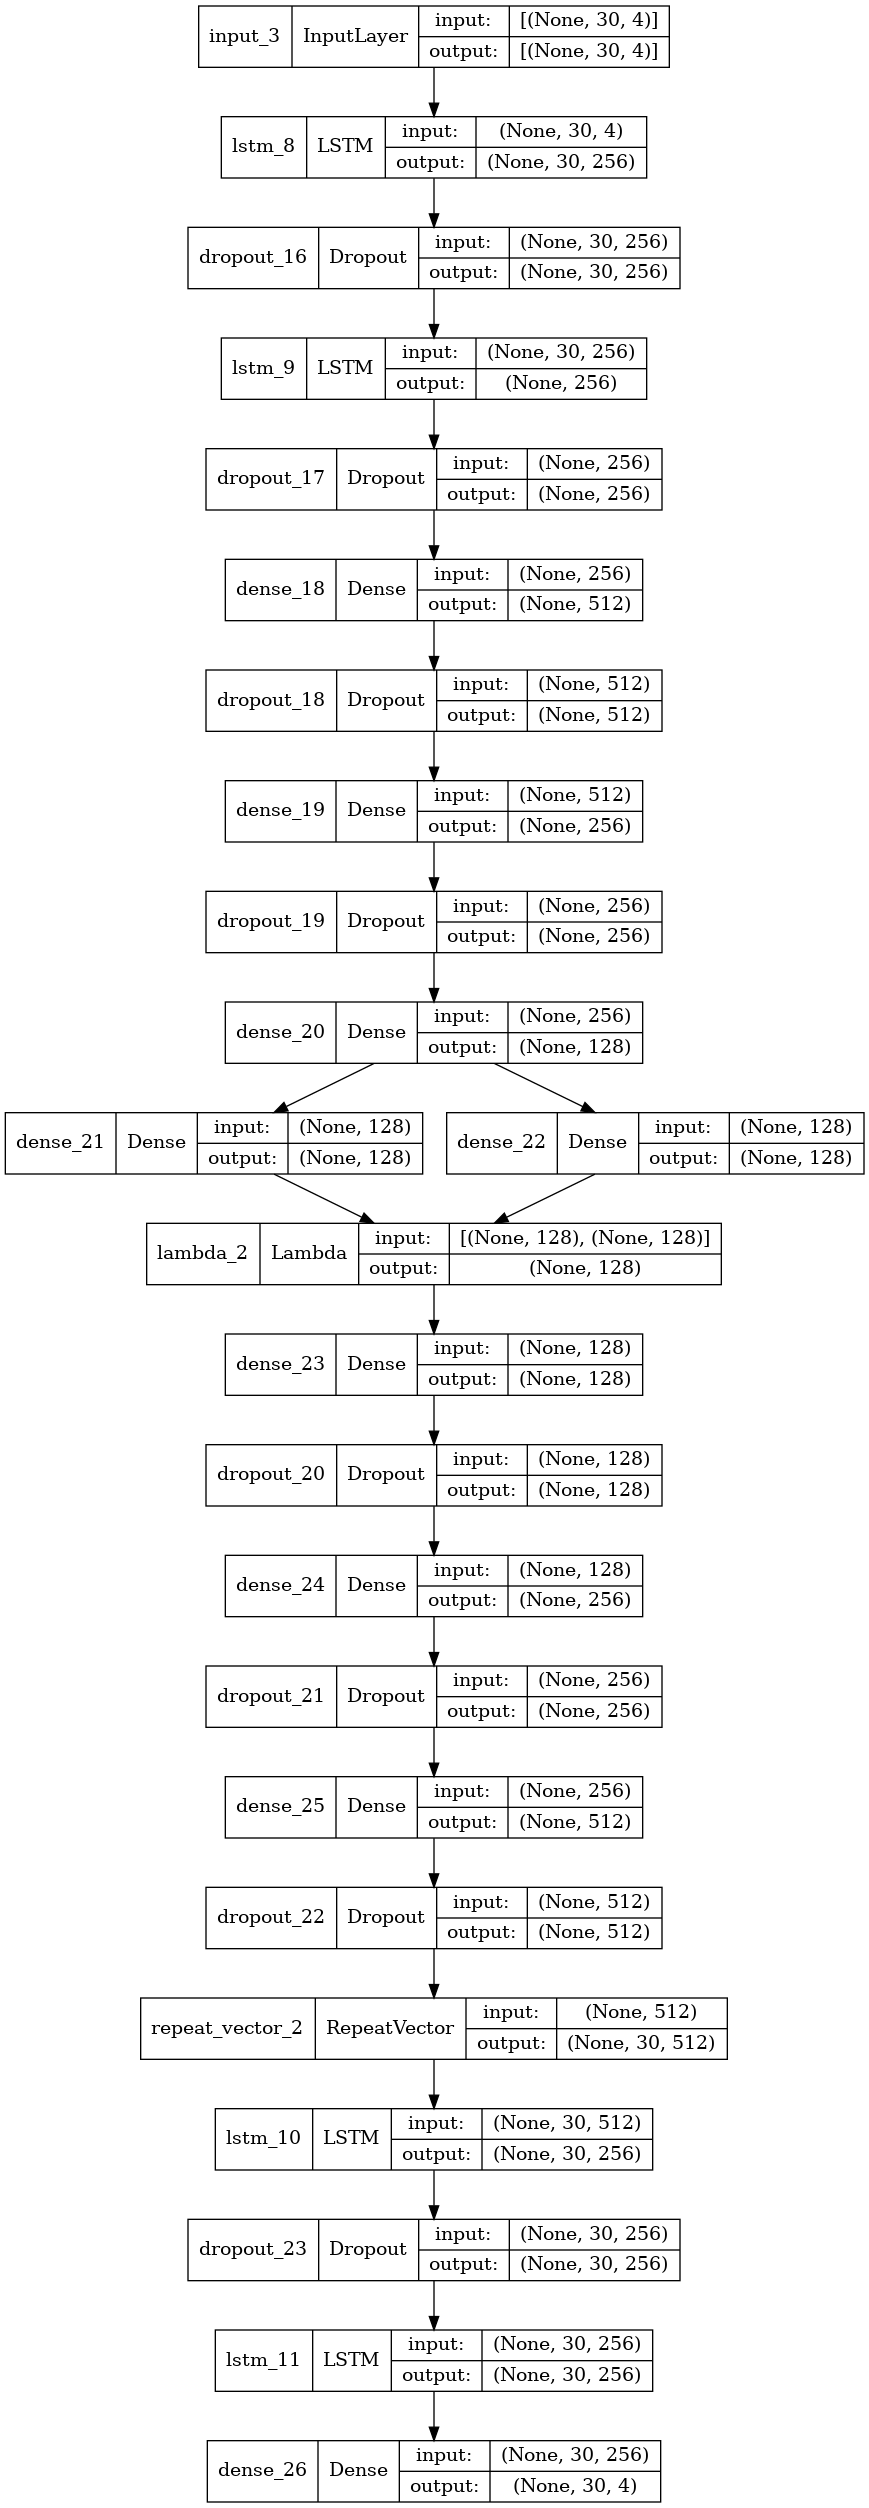
\includegraphics[height=0.9\textheight]{/task_2/vae.png}
		\caption{The VAE model}
		\label{task_2/vae}
	\end{figure}
	After the model definition, we fitted it for 100 epochs using a batch size of 32, keeping track of the MAE of the validation data used during training, in order to save only the best behaving model; this was done using a Model Checkpoint as callback to the fitting process.
	\begin{figure}
		\centering
		\includegraphics[width=\linewidth]{/task_2/loss&mae.png}
		\caption{The VAE loss and MAE}
		\label{task_2/loss&mae}
	\end{figure}
	
	\subsection{Evaluation}
	Talking about evaluation and results
	
	\newpage
	
	\section{Conclusions}
	conclusions about this task
	
\end{document}